% ------- Create Preamble ------------
\documentclass [12pt]{article} 
\usepackage[a4paper]{geometry} 
\usepackage{amsmath, amsthm, amssymb, amsfonts}
 \usepackage{graphicx,epsfig}
\usepackage{booktabs} 
\usepackage{pslatex} 
\usepackage{caption} 
\usepackage{setspace} 
\usepackage{hyperref} 
\usepackage{multicol, multirow}
\usepackage{graphicx,epsfig}
\usepackage{booktabs}
\usepackage{pslatex}
\usepackage{caption}
\usepackage{setspace}
\usepackage{hyperref}
\usepackage{multicol}
\usepackage{textgreek}
\usepackage{pdfpages}
\usepackage{apacite}
\usepackage{float}
\usepackage{natbib} % For references
\bibpunct{(}{)}{;}{a}{}{,} % Reference punctuation
\def\citeapos#1{\citeauthor{#1}'s (\citeyear{#1})}
\newtheorem{hypothesis}{Hypothesis}
\newtheorem{nullhypothesis}{Null Hypothesis}
\usepackage{xcolor}
\hypersetup{
    colorlinks,
    linkcolor={blue!50!blue},
    citecolor={black!50!black},
    urlcolor={blue!80!blue}
}

\usepackage{tikz}
\usetikzlibrary{shapes.geometric, arrows}
\tikzstyle{startstop} = [rectangle, rounded corners, minimum width=3cm, minimum height=1cm,text centered, draw=black, fill=white]
\tikzstyle{io} = [rectangle, rounded corners, minimum width=3cm, minimum height=1cm,text centered, draw=black, fill=white]
\tikzstyle{io2} = [rectangle, rounded corners, minimum width=3cm, minimum height=1cm,text centered, draw=black, fill=white]
\tikzstyle{arrow} = [thick,->,>=stealth]
%---Set up author and title page
\singlespace
\title{Giving the leaves back to the tree: Using random forest models for imputation}
\author{Damon C.\ Roberts\footnote{Ph.D Student,
Department of Political Science, University of Colorado Boulder, UCB 333, Boulder, CO 80309-0333. Damon.Roberts-1@colorado.edu. \newline \textbf{Acknowledgements:} I would like to thank Andrew Q. Philips for our many conversations and his advice for this manuscript. I would also like to thank Andrew Baker for encouraging me to take the time and the space to write this manuscript. \newline \textbf{Replication Code} can be found at: https://github.com/DamonCharlesRoberts/imputation-with-random-forests}}

%set up document
\date{}
\begin{document}
\maketitle
\begin{abstract}
Other fields such as the Biomedical Sciences and Computer Science use and advocate for Random Forest models as a flexible tool for imputing sparse datasets. To my knowledge, the use of this tool has yet to enjoy wide usage in political science. Implementations of Random Forest models in the multiple imputation paradigm referred to as MICE (or as it is sometimes called fully conditional specification) are flexible and loosen the distributional assumption required for popular techniques used by political scientists. Additionally, implementation of these models is relatively easy. The MICE implementation in Python, R, and STATA include Random Forest models for the use of imputation. In this manuscript, I use simulated and real world survey data to examine the conditions under which Random Forest models perform well. I compare its performance to that of AMELIA and of other MICE models.
\end{abstract}

\newpage
\doublespace
\newpage
\section{Introduction}

Missing values are common in social science data. King and colleagues \citep{king_et-al_2001} estimate that political scientists lose about one-third of their data in their complete case regression analyses due to missing data. There are many reasons as to why missing values arise in our data. In surveys, these are referred to item-nonresponse and pose threats to unbiased estimates to public opinion research when researchers utilize listwise deletion (LWD) in their regression analyses \citep{weisberg_2005}; particularly when the researcher is able to predict the cause of the missingness with an observed cause - which the data are referred to as "missing at random" \citep{king_et-al_2001}.\footnote{Which is a common occurance, more so than missigness caused entirely by random chance - which, if this condition is met, gives unbiased estimates with LWD.} More generally, missing values come about in other types of data as a result of the unit's (e.g. country, respondent, politician) attempt to obfuscate information, data collector error, or researcher error.  When common and not from a stochastic data generating process (DGP), missing data pose threats to causal inference either through model identification with non-full rank matracies or sample representativeness. 

Unsurprisingly a number of political scientists generate tools and learn from other fields to deal with these challenges. Many of the most popular approaches to imputation carry assumptions that scholars have to satisfy. There are four primary approaches that political scientists use in dealing with missing data: (1) listwise deletion or complete case analysis (LWD), (2) simple mean or median based imputation, (3) hot deck or regression based imputation, or (3) multiple imputation (MI). In this manuscript, I advocate for the application of flexible machine learning approaches to imputing missing values using a variant of the MI framework called Multiple Imputation through Chained Equations (MICE). Those who use machine learning models for predictive regressions often use random forest models due to their flexibility as a result of their fully non-parametric nature. Fields like the biomedical sciences treat missing values as out-of-sample predictions that random forest models predict. 

Not only do other fields use random forest models for imputation, but it is relatively easy to implement as well with contemporary computational and software capabilities. Using the Multiple Imputation by Chained Equations (MICE) paradigm, there are a number of single-line implementations in common data analysis software such as STATA, R, and Python \citep[see][]{buuren_goothuis-oudshoorn_2011}. 

This manuscript compares the utility of random forest models for imputation to other common imputation tools used in political science. The next section provide more details on the common imputation approaches that political scientists currently use. Following that, the following section describes random forest models and their utility for predicting missing data. I then move into applied examples where I compare the performance of these random forest models to other common imputation approaches on simulated data and an applied example with the 2017-2020 panel of the World Values Survey. I then close with a discussion of recommendations for when one should use the reigning popular techniques or the random forest application. 

\section{Common Approaches to dealing with missing data, imputation, and MI in Political Science}
	\subsection{MCAR, MAR, and MNAR}
Missing data arise in different forms. There are three key ways researchers describe missing data. The first form that missing data take are Missing Completely At Random (MCAR). This means that the data generating process for the missingness is random - there are no observed or unobserved causes of missingness. The second form that missing data take are Missing At Random (MAR). In MAR, these data are missing due to some observed cause. Some argue that MAR is much more common given the state of how large most contemporary social science data sets are \citep{schunk_2008}. The third form that missing data take are Missing Not At Random (MNAR).\footnote{Sometimes called Non-ignorable (NI).} MNAR happens when the cause for missingness is explained both by observed and unobserved causes. Given that missing data take different forms, researchers use a few different approaches to deal with these data.
 	\subsection{Dealing with missingness}
At the time of writing King and colleagues \citeyearpar{king_et-al_2001} estimated that $94\%$ of political scientists use LWD to deal with missing data. In short, LWD does not seek to impute missing values. Instead, if the DV or any of the covariates in a regression model for a given observation are missing, the researcher does not include that observation in the analysis. Traditionally, scholars argue that LWD performs best (in terms of reducing the resulting bias in the researcher's subsequent regression models) when the data are MCAR. If the data are MAR or MNAR, deleting observations with missing data are generating bias in one's regression estimates through a form of unit non-response bias \citep[see][]{weisberg_2005}.\footnote{Many others make a similar argument, but with different, non-survey, terminology \citep[see][to name a few]{king_et-al_2001, schunk_2008, azur_et-al_2011}.} A meta-analysis of comparative and international political economy papers that use LWD demonstrates that political scientists have much, upwards of $50\%$, more Type I error than we would expect as a result of how we implement LWD \citep{lall_2016}. Others push against this claim and instead argue that LWD does not inherently generate bias for non-MCAR data, but that researchers neglect to control for the cause of MAR or MNAR \citep{arel-bundock_pelc_2018}. 

Like LWD, simple imputation techniques like mean- and median-based imputation do not reduce the chances of biased regression estimates. These approaches sometimes called interpolation and extrapolation are commonly used with panel data. If you have missing data for an observation in one panel, you can take the same observations' response in a previous panel and a latter panel. You then take the mean or the median of that particular observation for that variable. Other approaches seek to reduce this MAR-based bias through conditioning on other variables.

Hot Deck approaches to imputing missingness are regression-based in that they define the dependent variable as the one the researcher is attempting to impute and use variables thought to predict the cause of missingness in MAR contexts \citep{schunk_2008}. You often use a minimal number of variables to condition on in this approach. In many cases, the precise mechanism generating missingness is often quite difficult to triangulate. As a result, if you fail to provide the right model specification when the data are MAR, you still often end up with biased regression estimates anyhow. 

MI seeks to solve this issue through using the entire dataset for imputing missing values \citep{rubin_1996}. This approach uses the other variables in the dataset to generate a joint posterior distribution of all possible missing values for that particular observation. Many assume that most social science data sets are sufficiently large enough to condition on the mechanism generating MAR \citep{schunk_2008}. Unlike the other approaches, MI also generates uncertainty around the imputed values \citep{rubin_1996} which enables the researcher to be more transparent about the validity of those imputed values and to include that uncertainty in the researcher's subsequent statistical analyses \citep{king_et-al_2001, von-hippel_2015}. A very popular implementation of MI in political science is Honaker, King, and Blackwell's \citeyearpar{honaker_et-al_2011} AMELIA II software \citep{lall_2016}. This useful tool provides a computationally fast and simple process for imputation. Compared to the other approaches to missing data, AMELIA II performs quite well \citeyearpar{honaker_et-al_2011, kropko_et-al_2014}. MI, however, often requires a set of distributional assumptions for the joint distribution - often the multivariate normal \citep{honaker_et-al_2011}.

There is a variant to MI which seeks more computational efficiency and loosens some of the distributional assumptions required. This variant is called Multiple Imputation through Chained Equations (MICE). MICE performs quite well for large imputation tasks. MI struggles to impute values when there is missingness in the other variables of the dataset \citep{kropko_et-al_2014} - which is quite common. This is because the way that the joint distribution is constructed. If there are missing values in the variables to be included in the joint distribution, this introduces bias in that distribution. MICE tries to get around this problem in a few steps as described by Azur and colleagues \citep{azur_et-al_2011}. First, it performs a simple imputation for every missing value in the entire dataset. These are the placeholder values. The second step involves identifying one variable to impute. Once this has been done, it then removes those placeholder values. The third step then involves regressing the observed values of the variable on the other variables in the model and replace the predicted values generated from the regression model for the missing values. The fourth step is to then repeat steps two and three for each variable in the data set with missing values - this constitutes a single iteration. As a fifth step, you perform between five and ten iterations.\footnote{Though, the exact number of recommended iterations used in MICE are still up for debate \citep[see][]{buuren_goothuis-oudshoorn_2011, azur_et_al_2011}.} 

The regression models that one may use in MICE are as numerous as the regression models a researcher may choose from when engaged in a statistical analysis. This means, however, that the assumptions and the performance of the model one uses for the imputation are the same as they are in standard statistical analyses. Selection of the model to use in MICE should be carefully thought out. One valuable model for generating out-of-sample predictions is a form of ensemble machine learning model called Random Forests. 
\section{The utility of random forest models for imputing political science data}
Random forest models are concerned with calculating a fixed out of sample prediction. This is in line with the argument that multiple imputation  should not be evaluated on the model's correctness but on the model's ability to predict a fixed (true) value \citep{rubin_1996}. Here, I think of missing data as the out of sample predictions that are intended to be estimated. With random forest models, you train the model on a training data set (often randomly generated through cross validation) and then fit the model on the testing set \citep{hastie_et-al_2009}. OLS models often perform relatively poorly on making out-of-sample predictions as they are BLUE assuming the data on hand are relatively representative of the population. As we have MAR data, this assumption likely fails and any out-of-sample predictions are likely to be biased. OLS may also generate out-of-bounds predictions for non-continuous data \citep{long_1997,gelman_et-al_2021}. 

There are other models which provide within-bounds predictions such as logistic models, however, as generalized linear models, they still assume a linear functional form. Random forest models both provide within-bounds predictions and they are fully non-parametric \citep{hastie_et-al_2009}; meaning they do not assume a functional form and consequently a joint distribution. 

On other performance metrics, random forest models, as a ensemble method, provide much more accurate predictions than single models, such as CART \citep{montgomery_olivella_2018}. Rather than generating the single estimate from a single model, ensemble models like random forests, calculate multiple models and learn from their performance. Specifically, random forest models takes bootstrapped samples of the dataset and fits multiple trees (a single tree model being one which successively fit models that refine a trade-off between the bias and efficiency).

In the context of MICE, political scientists can use random forest models to make accurate predictions with fewer assumptions and leniency in terms of conditioning on the cause of MAR in the data set. Recall that within each MICE iteration, one performs a model predicting (imputing) a missing value based on the other variables in the dataset. Explicitly, this means that you are running a model per variable with missing data. Given that random forests are non-parametric, within each MICE iteration, the relationship between the variable to be imputed and those used to make the predictions can be non-linear and can take many different distributional forms. This is a significant advancement on traditional MI which assumes a joint normal distribution. Additionally, this is an advancement on other MICE models which may assume linear relationships. Furthermore, using random forests in MICE has the advantage over hot deck procedures for those unsure about the precise DGP for MAR in a variable. Figure \ref{fig:1} provides a brief summary of using random forests to impute missing values with MICE. 
\begin{figure*}
	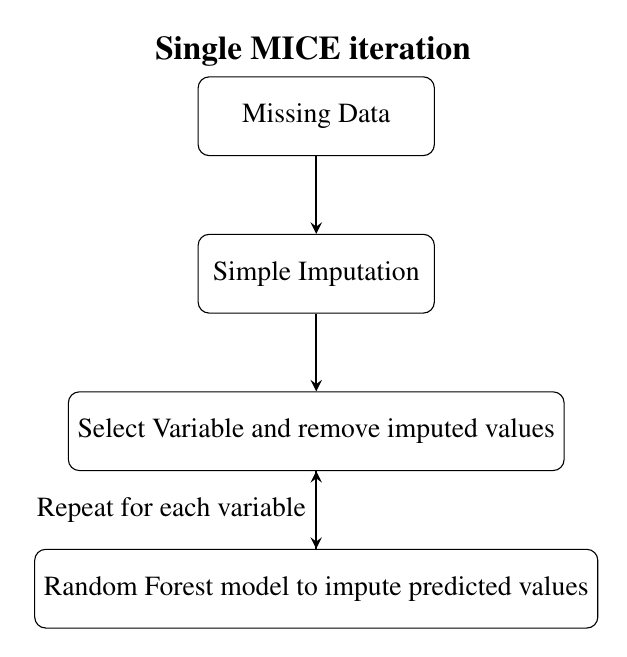
\begin{tikzpicture}[node distance = 2cm]
	\node (start) [startstop] {Missing Data};
	\node (in1) [io, below of=start]{Simple Imputation};
	\node (in2) [io, below of=in1]{Select Variable and remove imputed values};
	\node (in3) [io, below of=in2]{Random Forest model to impute predicted values};
	\draw [arrow] (in3) -- node[anchor = east] {Repeat for each variable} (in2);
	\draw [arrow] (start) -- (in1);
	\draw [arrow] (in1) -- (in2);
	\draw [arrow] (in2) -- (in3);
	\node [above, font = \large\bfseries] at (current bounding box.north) {Single MICE iteration};
\end{tikzpicture}
	\caption{MICE with Random Forest models}
	\label{fig:1}
\end{figure*}


For example, say we have a $3x3$ matrix, $m$, where:
\begin{equation*}
m = 
\begin{bmatrix}
	NA & 1 & 2 \\
	1 & NA & 2 \\
	1 & 2 & NA	
\end{bmatrix}
\end{equation*}
 The first step  would be to do a simple imputation that returned: 
 \begin{equation*}
 	m = \begin{bmatrix}
 		\textbf{1.5} & 1 & 2 \\
 		1 & \textbf{1.5} & 2 \\
 		1 & 2 & \textbf{1.5}
 		\end{bmatrix}	
 \end{equation*}

The second step would be to remove $m_{11}$ yielding:
\begin{equation*}
	m = 
	\begin{bmatrix}
		NA & 1 & 2 \\
		1 & \textbf{1.5} & 2 \\
		1 & 2 & \textbf{1.5}
	\end{bmatrix}
\end{equation*}
And then running a random forest model to predict the value of $m_{11}$.

This second step yields:
\begin{equation*}
	m = \begin{bmatrix}
 	1.4 & 1 & 2 \\
 	1 & \textbf{1.5} & 2 \\
 	1 & 2 & \textbf{1.5}	
 \end{bmatrix}
\end{equation*}

This is then repeated for the other columns in the matrix. Once completed for each column in the matrix, this constitutes 1 iteration. This is then done between five and 10 more times. This then gives you a distribution of imputed values for each cell that were originally missing. 
 
In the next section, I illustrate the use of random forest models for political scientists by demonstrating a simulated and real-world application of a random forest implementation of MICE. The next section also compares this implementation's performance to that of other common approaches to handling missing data in political science. 

\section{Application of MICE with random forests}
	\subsection{Simulated Data}
	To give an example of how this procedure works, I start with a controlled dataset. I simulated two datasets. The first dataset has three variables where the means and the covariance matrix were randomized. The second dataset has ten variables where the means and the covariance matrix were randomized. Each of these datasets have 1000 observations. These represent my complete simulated datasets.
	
	With these two datasets, I also introduced MCAR, MAR, and MNAR \footnote{The code used to introduce the randomness can be found in the Github repository containing the replication materials). This yields six total simulated datasets. 
	
	While multiple imputation is most effective for data that are MAR, I wanted to demonstrate the performance of this procedure to the others in different circumstances.
	\begin{enumerate}
		\item Distributional Performance (MVN versus other distributions)
		\item MCAR, MAR, MNAR Performance
		\item Variable structure (i.e. continuous, ordinal, nominal, discrete)??
	\end{enumerate}
	\subsection{In the wild: World Values Survey 2017-2020 Panel}
\section{Conclusion}
The imputation model used here is a form of multiple imputation. As a result, it does have its limitations. As King and colleagues \citeyearpar{king_et-al_2001} outline, listwise deletion preforms better than MI when:
	\begin{quote}
	(1) The analysis model is conditional on X ..., and the functional form is known to be correctly specified ... (2) There is NI [MNAR] missingness in X, so that [the algorithm] can give incorrect answers, and no Z variables are available that could be used in an imputation stage to fix the problem. (3) Missingness in X is not a function of Y, and unobserved omitted variables that affect Y do not exist... (4) The number of observations left after listwise deletion should be so large that the efficiently loss from listwise deletion does not counterbalance the biases induced by the other conditions.
	\end{quote}
Random forest models not for multiple imputation are especially prone to a decline in performance when X is sparse. Given that this already is a problem for MI models, this is certainly a significant drawback to the implementation of random forests for MI. If one has a sparse data set, using random forest models for MI should certainly be reconsidered. 

\bibliographystyle{apsr}
\bibliography{/Users/damonroberts/Dropbox/bibliographies/methods/measurement_error.bib,/Users/damonroberts/Dropbox/bibliographies/methods/robustness.bib,/Users/damonroberts/Dropbox/bibliographies/methods/multiple_imputation.bib,/Users/damonroberts/Dropbox/bibliographies/methods/random_forests.bib,/Users/damonroberts/Dropbox/bibliographies/methods/glm_mle.bib}
\end{document}
